\documentclass{article}
\usepackage{amsmath}
\usepackage{mathtools}
\usepackage[a4paper, total={6in, 8in}]{geometry}
\usepackage{amssymb}
\usepackage{color}
\usepackage{lscape}
\usepackage{listings}
\usepackage{xcolor}
\usepackage{float}
\usepackage{hyperref}
\usepackage{fancyhdr}
\pagestyle{fancy}

% Define the header
\fancyfoot[R]{Fernando Urbano}
\renewcommand{\footrulewidth}{0.2pt}

\fancyhead[L]{ECMA 31380 - Causal Machine Learning}
\fancyhead[R]{Homework 2}

\usepackage{graphicx}
\setlength{\parskip}{0.5em}
\setlength{\parindent}{0pt}
\renewcommand{\thesubsection}{\thesection.\alph{subsection}}
\newcommand{\divider}{\vspace{1em}\hrule\vspace{1em}}

\definecolor{codegreen}{rgb}{0,0.6,0}
\definecolor{codegray}{rgb}{0.5,0.5,0.5}
\definecolor{codepurple}{rgb}{0.58,0,0.82}
\definecolor{backcolour}{rgb}{0.95,0.95,0.92}

\lstdefinestyle{Rstyle}{
  backgroundcolor=\color{backcolour},   
  commentstyle=\color{codegreen},
  keywordstyle=\color{blue},
  numberstyle=\tiny\color{codegray},
  stringstyle=\color{codepurple},
  basicstyle=\ttfamily\footnotesize,
  breakatwhitespace=false,         
  breaklines=true,                 
  captionpos=b,                    
  keepspaces=true,                 
  numbers=left,                    
  numbersep=5pt,                  
  showspaces=false,                
  showstringspaces=false,
  showtabs=true,                  
  tabsize=2,
  language=R
}

\title{ECMA 31380 - Draft Final Project}
\author{Fernando Rocha Urbano}
\date{Autumn 2024}

% Define colors
\definecolor{codegreen}{rgb}{0,0.6,0}
\definecolor{codegray}{rgb}{0.5,0.5,0.5}
\definecolor{codepurple}{rgb}{0.58,0,0.82}
\definecolor{backcolour}{rgb}{0.95,0.95,0.92}

% Setup the listings package
\lstdefinestyle{mystyle}{
    backgroundcolor=\color{backcolour},   
    commentstyle=\color{codegreen},
    keywordstyle=\color{magenta},
    numberstyle=\tiny\color{codegray},
    stringstyle=\color{codepurple},
    basicstyle=\ttfamily\footnotesize,
    breakatwhitespace=false,         
    breaklines=true,                 
    captionpos=b,                    
    keepspaces=true,                 
    numbers=left,                    
    numbersep=5pt,                  
    showspaces=false,                
    showstringspaces=false,
    showtabs=false,                  
    tabsize=2
}

\newenvironment{colorparagraph}[1]{\par\color{#1}}{\par}
\definecolor{questioncolor}{RGB}{20, 40, 150}
\definecolor{tacolor}{RGB}{200, 0, 0}

\lstset{style=mystyle}

\begin{document}

\maketitle

\section{Causal Factor Investing: Can Factor Investing Become Scientific?}

Authors of factor models do not identify the causal graph consistent with the observed phenomenon, they justify their chosen model specification in terms of correlation and do not propose experiments for falsifying causal mechanisms.

Absent a causal theory, their findings are likely false, due to rampant backtest overfitting and incorrect specification choices.

Economists subscribe to the view that genuine science must produce refutable implifications.

In the absence of plausible falsifiable theories, researchers must acknowledge that they do not understand why the reported anomalies (risk premia) occur.

\subsection{Association vs Causation}

Two variables are statistically associated if:

$$
\mathbb{P}[X = x, Y = y] \neq \mathbb{P}[X = x] \times \mathbb{P}[Y = y]
$$

A variable $X$ is said to cause a variable $Y$ when $Y$ is a function of $X$ in the data generating process.

There is a difference between conditioning $X = x$ and setting. The idea of setting is an intervention.

The intervention means that you set the value of $X$, which is often represented with $do[X = x]$.

If $X$ does not cause $Y$:

$$
\mathbb{P}[Y = y \mid do[X = x]] = \mathbb{P}[Y = y]
$$

Even if:

$$
\mathbb{P}[Y = y \mid X = x] \neq \mathbb{P}[Y = y]
$$

For instance, if $Z$ causes $X$ and $Y$, $Z$ is considered a confounder, because it is the variable that introduces association between $X$ and $Y$, even though there is no relationship in the data generating process between $X$ and $Y$.

\begin{figure}[H]
  \centering
  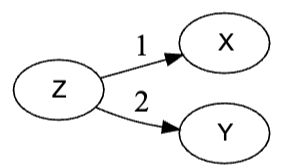
\includegraphics[width=100px]{draft-photos/confounder_variable.png}
  \caption{$Z$ confounder for $X$ and $Y$}
  \label{fig:confounder_variable}
\end{figure}

Causality is an extra-statistical concept, connected to mechanisms and interventions.

Causation does imply association because setting $X = x$ through an intervention is associated with the $Y = y$.

Causality is directional. The statement "$X$ causes $Y$" implies:

$$
\mathbb{P}[Y = y \mid do[X = x]] \neq \mathbb{P}[Y = y]
$$

But does not imply:

$$
\mathbb{P}[X = x \mid do[Y = y]] \neq \mathbb{P}[X = x]
$$

Association is not directional.

Studies designed to establish causality propose methods to nullify the bias of the ATT (SSB). These are:

\begin{enumerate}
  \item Intervention Studies (RCT): randomized controlled trials.
  \item Natural Experiments: when intervention studies are not possible (unfeasible, unethical). Units are assigned to the treatment and control groups determined randomly by Nature. Common examples of natural experiments include: (1) regression discontinuity design (RDD); (2) crossover studies (COS); and (3) difference-in-differences (DID) studies. The critical assumption behind RDD is that groups (a) and (b) are comparable in everything but the slight difference in the assignment variable, which can be attributed to noise. A COS is a longitudinal study in which the exposure of units to a treatment is randomly removed for a time, and then returned. COS assume that the effect of confounders does not change per unit over time.
  \item Simulated Interventions: researchers may still conduct an observational study that simulates a do-operation, with the help of a hypothesized causal graph. The hypothesized causal graph encodes the information needed to remove from observations the SSB introduced by confounders, under the assumption that the causal graph is correct.
\end{enumerate}

\subsection{Hypothesized Causal Graph}

A simulated intervention allows researchers to estimate the strength of a causal effect from observational studies. Second, a simulated intervention may help falsify a hypothesized causal graph, when the strength of one of the effects posited by the graph is deemed statistically insignificant.

In simulated interventions, the causal graph is part of the assumptions, and one cannot prove what one is assuming. The most a simulated intervention can achieve is to disprove a hypothesized causal
graph, by finding a contradiction between an effect claimed by a graph and the effect estimated
with the help of that same graph.

The latter differs from interventional studies and natural experiments. In those, subject to some
assumptions, a researcher can establish or falsify a causal claim without knowledge of the causal
graph. 

The most a simulated intervention can achieve is to disprove a hypothesized causal graph, by finding a contradiction between an effect claimed by a graph and the effect estimated with the help of that same graph. This power of simulated interventions to falsify causal claims can be very helpful in discovering through elimination the causal structure hidden in the data.

\subsection{Causal Discovery}

Can be defined as the search for the structure of causal relationships, by analyzing the statistical properties of observational evidence.

While observational evidence almost never suffices to fully characterize a causal graph, it often contains information helpful in reducing the number of possible structures of interdependence among variables.

In more recent years, scientists have developed numerous computational methods and algorithms for the discovery of causal relations, represented as directed acyclic graphs.

\begin{itemize}
  \item constraint-based algorithms
  \item score-based algorithms
  \item functional causal models
\end{itemize}

\subsubsection{Constraint-Based Algorithms}
The two most widely used are:

\begin{itemize}
  \item PC Algorithm: assumes that there are no latent (unobservable) confounders, and under this assumption the discovered causal information is asymptotically correct.
  \item FCI Algorithm: gives asymptotically correct results even in the presence of latent confounders.
\end{itemize}

\subsubsection{Score-based methods}
Score-based methods can be used in the absence of latent confounders. 

These algorithms attempt to find the causal structure by optimizing a defined score function. An example of a score-based method is the greedy equivalence search (GES) algorithm.

This heuristic algorithm searches over the space of Markov equivalence classes, that is, the set of causal structures satisfying the same conditional independences, evaluating the fitness of each structure based on a score calculated from the data.

\subsubsection{Functional Causal Models}

Causal graphs can also be derived from non-numerical data. For example, Laudy et al. [2022]
apply natural language processing techniques to news articles in which different authors express
views of the form $X \to Y$. By aggregating those views, these researchers derive directed acyclic
graphs that represent collective, forward-looking, point-in-time views of causal mechanisms.

\subsubsection{Machine Learning}

With ML, we can decouple the variable search from the specification search.

Examples include mean-decrease accuracy, local surrogate models, and Shapley values (López de Prado [2020, pp. 3-4], López de Prado [2022a]). 

\subsection{Blocked Paths}

In a graph with three variables $\{ X, Y, Z \}$, the variable $Z$ is:
\begin{itemize}
  \item Confounder with respect to $X$ and $Y$: when the causal relation has $X \leftarrow Z \to Y$
  \item Collider with respect to $X$ and $Y$: when the causal relation has $X \to Z \to \leftarrow Y$
  \item Mediator with respect to $X$ and $Y$: when the causal relation has $X \to Z \to Y$
\end{itemize}

A path is a sequence of arrows and nodes that connect the two variables $X$ and $Y$.

\begin{itemize}
  \item Directed path: path in which all arrows point in the same direction
  \item $X$ is ancestor of $Z$ in the path which starts with $X$ and ends with $Z$.
  \item $Z$ is descendant of $X$ in the path which starts with $X$ and ends with $Z$.
  \item A path between $X$ and $Y$ is blocked if either:
  \begin{itemize}
    \item the path traverses collider and the researcher has not conditioned on that collider or its descendants.
    \item the researcher conditions on a variable in the path between $X$ and $Y$, where the conditoned variable is not a collider.
  \end{itemize}
  \item Causal associations only flows along an unblocked directed path that starts in treatment $X$ and ends in outcome $Y$, denoted the causal path. Association implies causation only if all non-causal paths are blocked.
\end{itemize}

\subsection{Adjustments}
\subsubsection{Backdoor Adjustment}
A backdoor path between $X$ and $Y$ is an unblocked non-causal path that connects those two variables. The term backdoor is inspired by the fact that this kind of paths have an arrow pointing into the treatment ($X$).

This image has a backdoor path pointed in red (non-causal path) and a causal path in green.

Having this backdoor path is a problem due to association, not allowing to recover the true ATE.

Backdoor paths can be blocked by conditioning on a set of variables $S$ that satisfies the backdoor criterion. Meaning thta we want to control for observable confounders.

A set of variables $S$ satisfies the backdoor criterion with regards to treatment $X$ and outcome $Y$ if the following two conditions are true:
\begin{itemize}
  \item conditioning on $S$ blocks all backdoor paths between $X$ and $Y$ (blocks all non-causal paths).
  \item $S$ does not contain any descendants of $X$ (keeps open all causal paths).
\end{itemize}

Then, $S$ is a sufficient adjustment set, and the causal effect of $X$ on $Y$ can be estimated as

$$
\mathbb{P}[Y(x) = y] = \sum_s \mathbb{P}[Y(x) = y \mid X = x, S = s] \mathbb{P}[S = s]
$$

\begin{figure}[H]
  \centering
  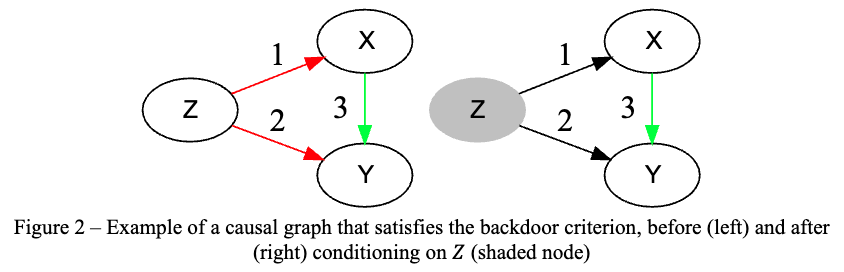
\includegraphics[width=250px]{draft-photos/backdoor_adjustment.png}
  \caption{Backdoor Adjustment}
  \label{fig:backdoor_adjustment}
\end{figure}

\subsubsection{Backdoor Adjustment: Another Explanation}

\url{https://www.youtube.com/watch?v=U1S8Rq8IcrY}

We want to block the $W_1$ and $C$ that are non causal associations.

\begin{figure}[H]
  \centering
  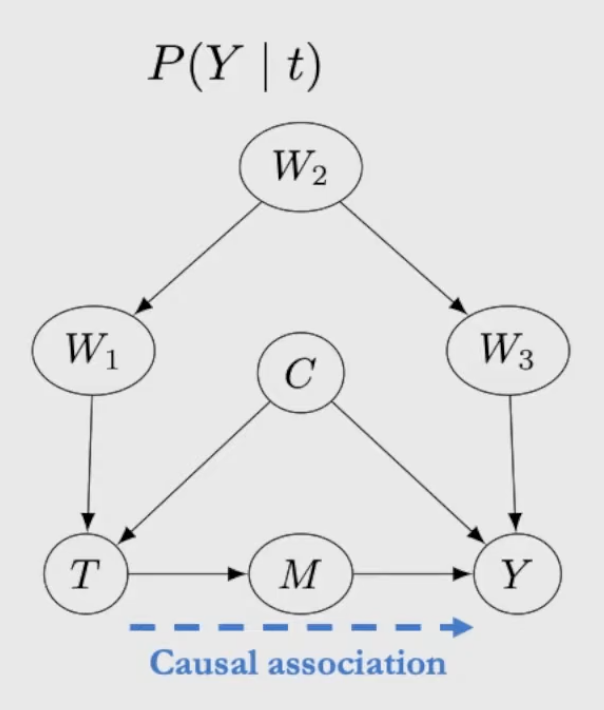
\includegraphics[width=250px]{draft-photos/backdoor_adjustment_explained.png}
  \caption{Backdoor Adjustment}
  \label{fig:backdoor_adjustment_explained}
\end{figure}

Our end goal is to find the interventional distribution of $Y(t)$.

\begin{figure}[H]
  \centering
  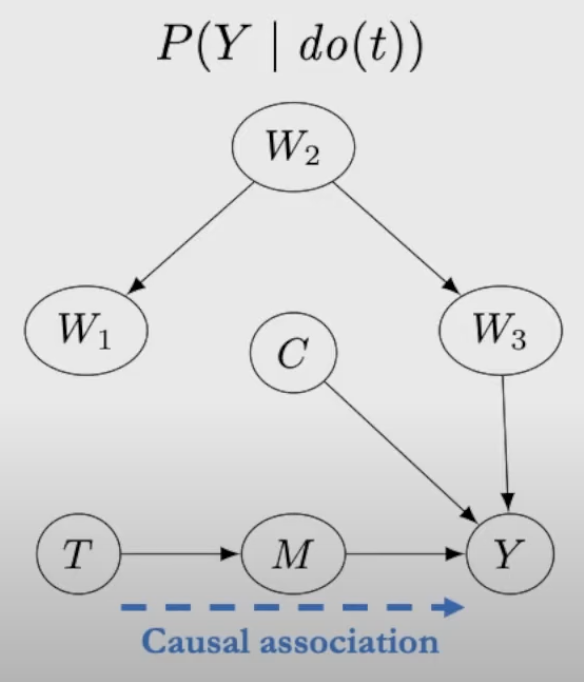
\includegraphics[width=250px]{draft-photos/backdoor_adjustment_explained_goal.png}
  \caption{Backdoor Adjustment}
  \label{fig:backdoor_adjustment_explained_goal}
\end{figure}

Nonetheless, this is not doable in data if, given that it is an intervention.

Thus, we must find $mathbb{P}[Y \mid t, W_2, c]$ or $mathbb{P}[Y \mid t, W_1, c]$ or $mathbb{P}[Y \mid t, W_3, c]$.

\begin{figure}[H]
  \centering
  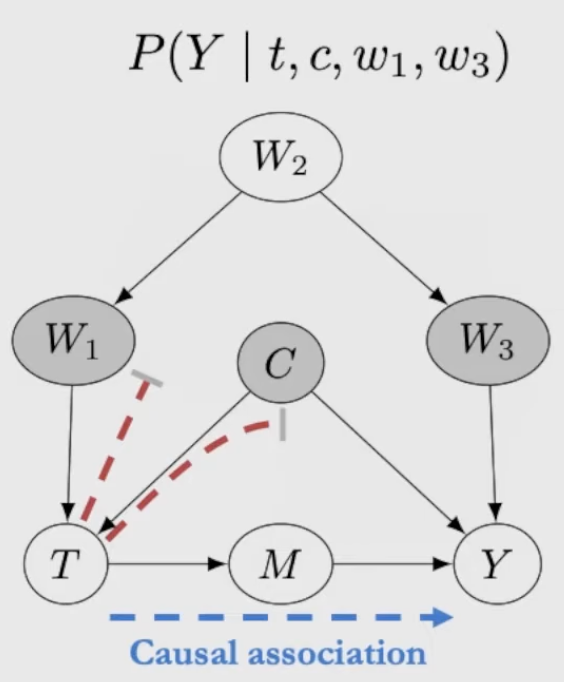
\includegraphics[width=250px]{draft-photos/backdoor_adjustment_explained_solution.png}
  \caption{Backdoor Adjustment}
  \label{fig:backdoor_adjustment_explained_solution}
\end{figure}

\begin{figure}[H]
  \centering
  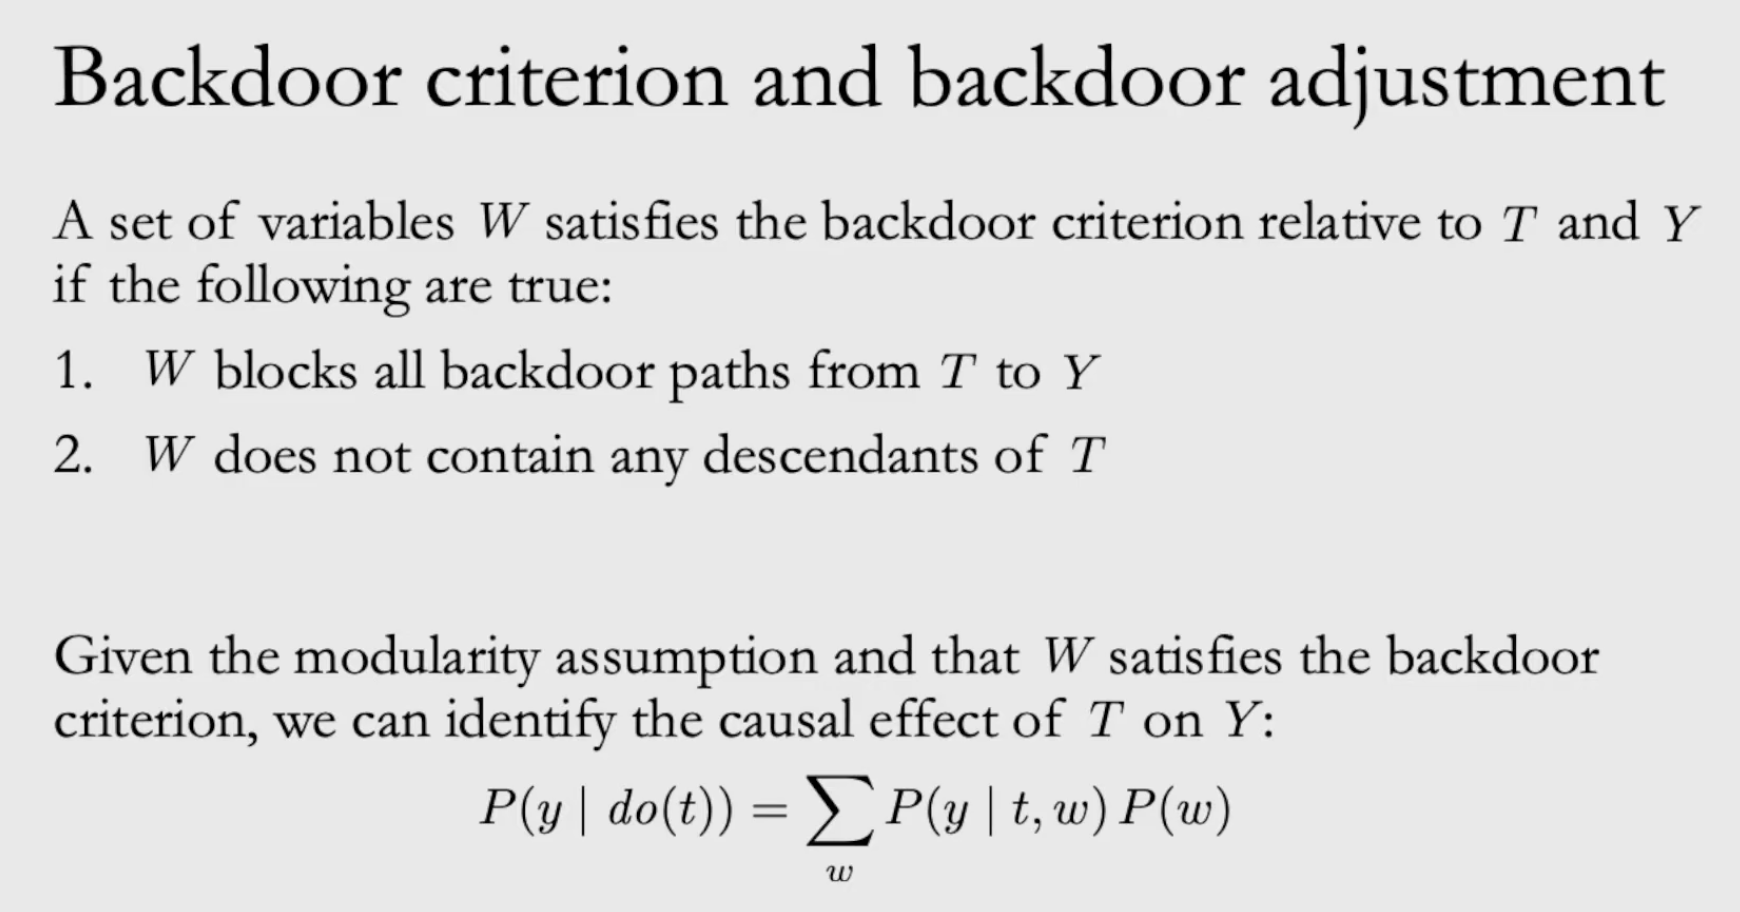
\includegraphics[width=250px]{draft-photos/backdoor_adjustment_explanation.png}
  \caption{Backdoor Adjustment}
  \label{fig:backdoor_adjustment_explanation}
\end{figure}

\begin{figure}[H]
  \centering
  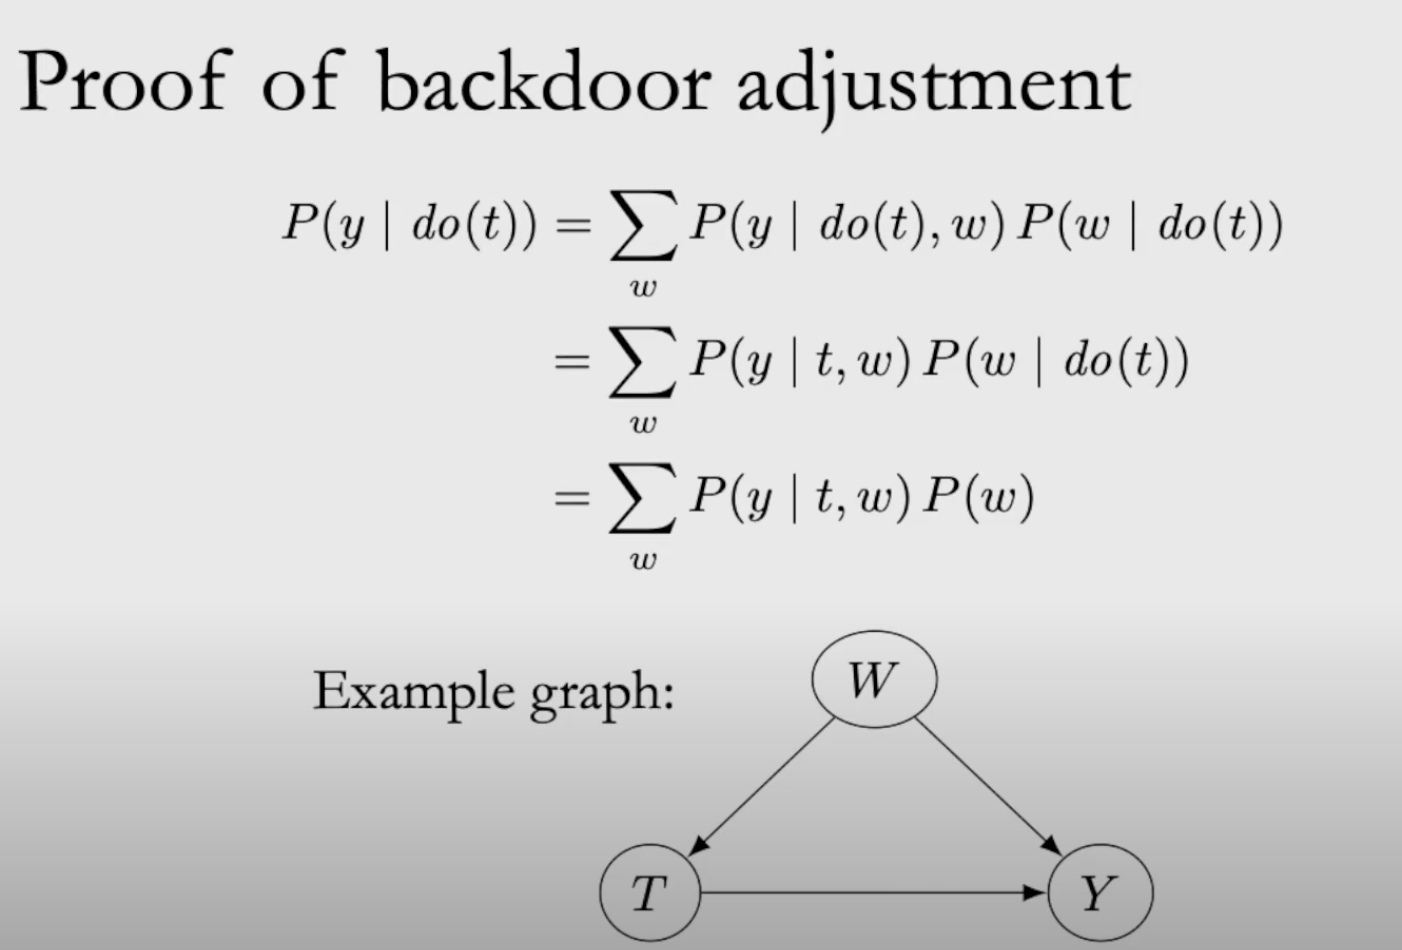
\includegraphics[width=250px]{draft-photos/backdoor_adjustment_explanation2.png}
  \caption{Backdoor Adjustment}
  \label{fig:backdoor_adjustment_explanation2}
\end{figure}

The backdoor criterion is often related to "d-separation".

it is very important that the set of variables used as backdoor blockers do not contain any descendants of the treatment.

Meaning that:

$$
Y \perp T | S
$$

Where $S$ is again the set of variables used as backdoor blockers.

\subsubsection{Front-Door Adjustment}

Sometimes researchers may not be able to condition on a variable that satisfies the backdoor criterion. That is such a case when the variable is latent (unobservable).

A causal approach can be achieved with a mediator.

A set of variables $S$ satisfies the front-door criterion with regards to treatment $X$ and outcome $Y$ if the following three conditions are true:

\begin{itemize}
  \item all causal paths from $X$ to $Y$ go through $S$
   \item there is no backdoor path between $X$ and $S$
  \item all backdoor paths between $S$ and $Y$ are blocked by conditioning on $X$.
\end{itemize}

\begin{figure}[H]
  \centering
  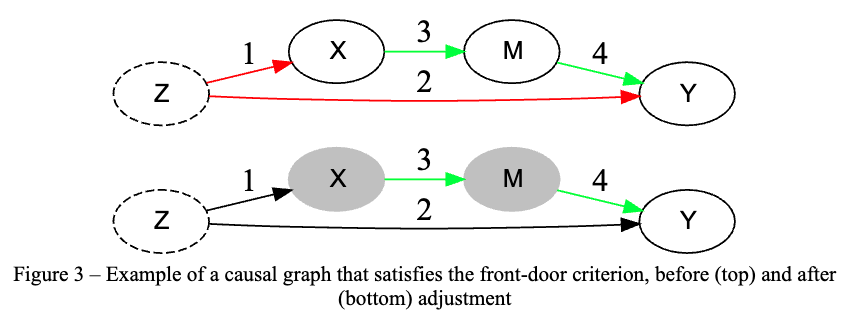
\includegraphics[width=250px]{draft-photos/frontdoor_adjustment.png}
  \caption{Frontdoor Adjustment}
  \label{fig:frontdoor_adjustment}
\end{figure}

Then, $S$ is a sufficient adjustment set, and the causal effect of $X$ on $Y$ can be
estimated as:

$$
\mathbb{P}[Y(x) = y] = \sum_s \mathbb{P}[S = s \mid X = x] \sum_{x'} \mathbb{P}[Y = y \mid X = x', S = s] \mathbb{P}[X = x']
$$

\subsubsection{Front-Door Adjustment: Another Explanation}

Recalling the backdoor adjustment, we use descendent variable to $T$ and $Y$ to correct the bias.

Nonetheless, lets say that those variables are not available (latent).

\begin{figure}[H]
  \centering
  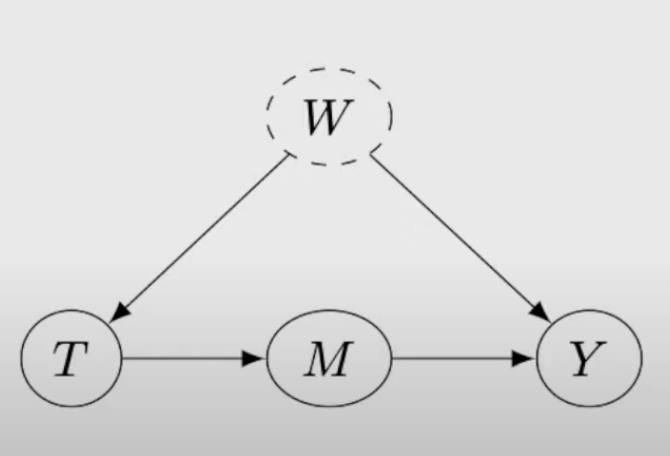
\includegraphics[width=250px]{draft-photos/frontdoor_adjustment_explained.png}
  \caption{Frontdoor Adjustment}
  \label{fig:frontdoor_adjustment_explained}
\end{figure}

Now, if we only focus on $M$, we can get a better perspective.

Meaning that we have to understand the causal association of $T$ to $M$ and the causal association of $M$ to $Y$.

\begin{figure}[H]
  \centering
  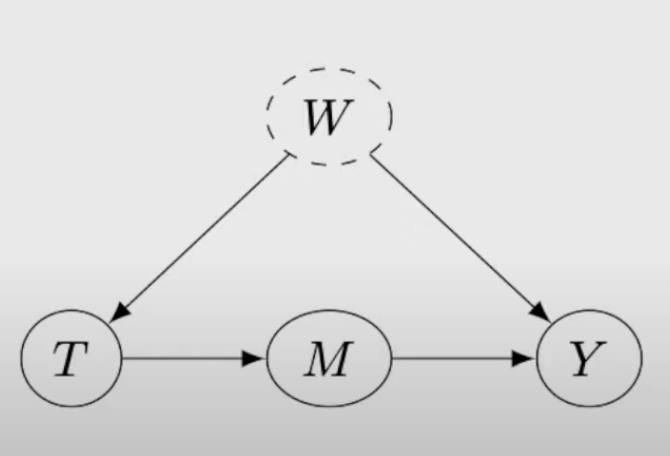
\includegraphics[width=250px]{draft-photos/frontdoor_adjustment_explained.png}
  \caption{Frontdoor Adjustment}
  \label{fig:frontdoor_adjustment_solution}
\end{figure}

The first step is to identify the causal effect of $T$ on $M$: here there is no backdoor path, therefore, the step is quite simple.

\begin{figure}[H]
  \centering
  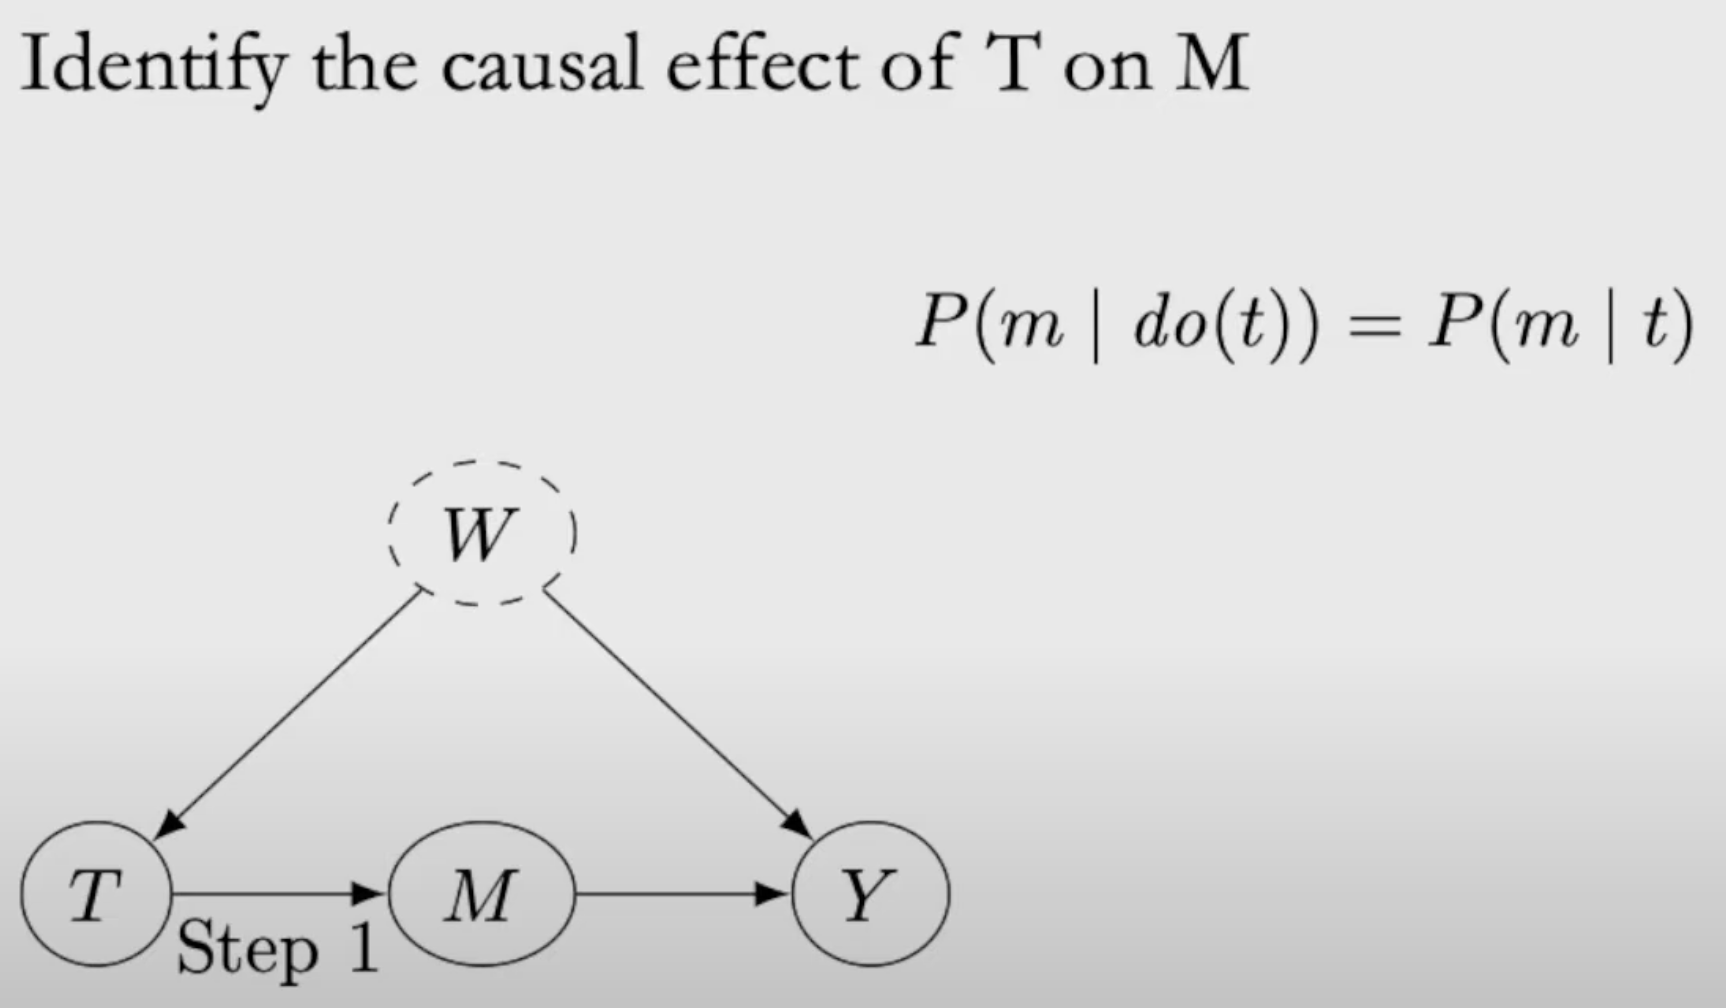
\includegraphics[width=250px]{draft-photos/frontdoor_adjustment_explanation.png}
  \caption{Frontdoor Adjustment}
  \label{fig:frontdoor_adjustment_explanation}
\end{figure}

The second step is identify the causal effect of $M$ on $Y$: here there is a backdoor path. Thus, we have to condition of $T$ to account for that.

\begin{figure}[H]
  \centering
  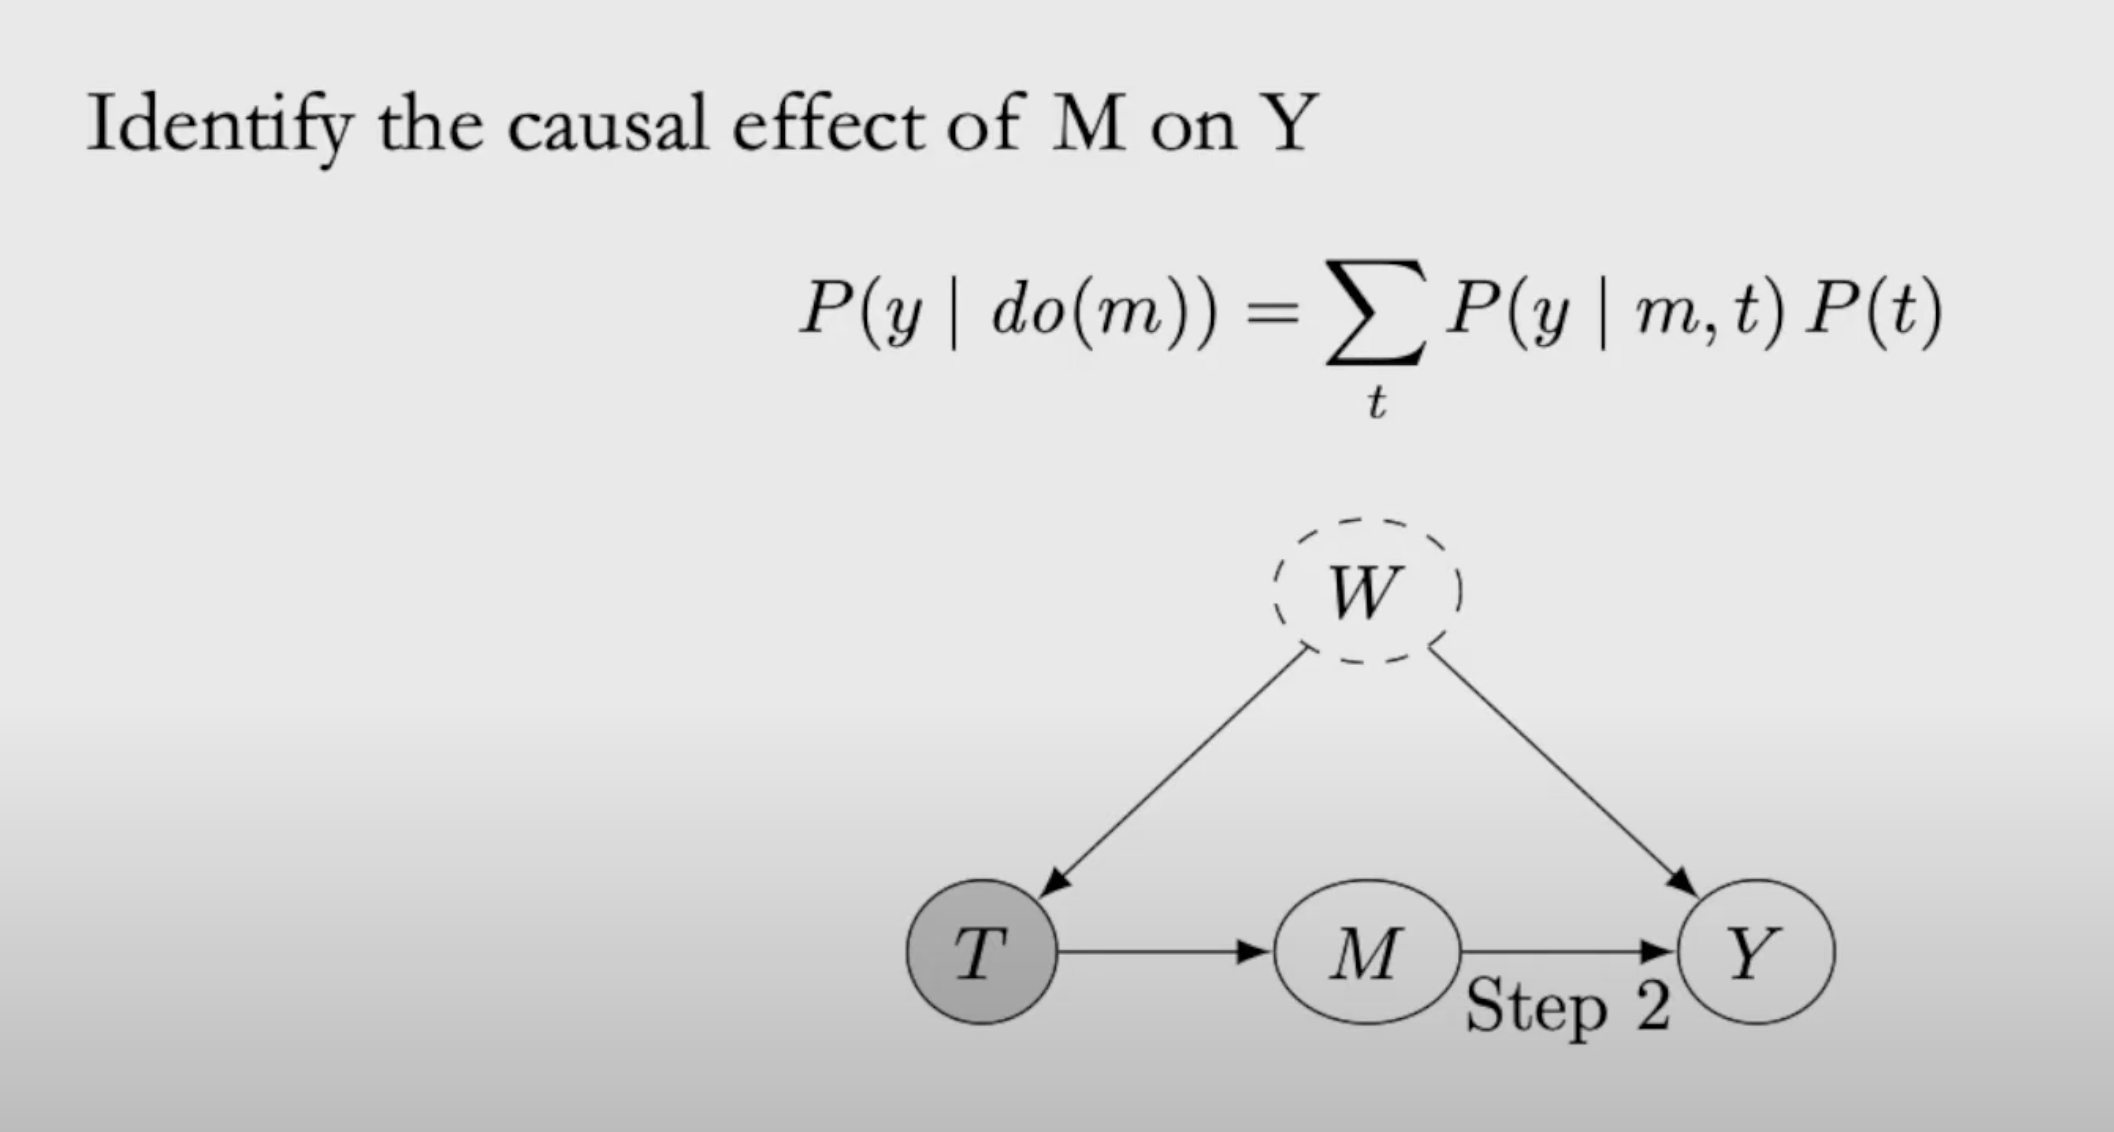
\includegraphics[width=250px]{draft-photos/frontdoor_adjustment_explanation2.png}
  \caption{Frontdoor Adjustment}
  \label{fig:frontdoor_adjustment_explanation2}
\end{figure}

The third step is to combine.

We use the causal association of $\mathbb{P}[m(t)]$ (step 1) and the $\mathbb{P}[y(m)]$.

Thus:

\begin{align*}
  \mathbb{P}[y(t)]
  &= \sum_m \mathbb{P}[m(t)] \mathbb{P}[y(m)] \\
  &= \sum_m \mathbb{P}[m \mid t] \sum_{t'} \mathbb{P}[y | m, t'] \mathbb{P}[t'] \\
\end{align*}

\begin{figure}[H]
  \centering
  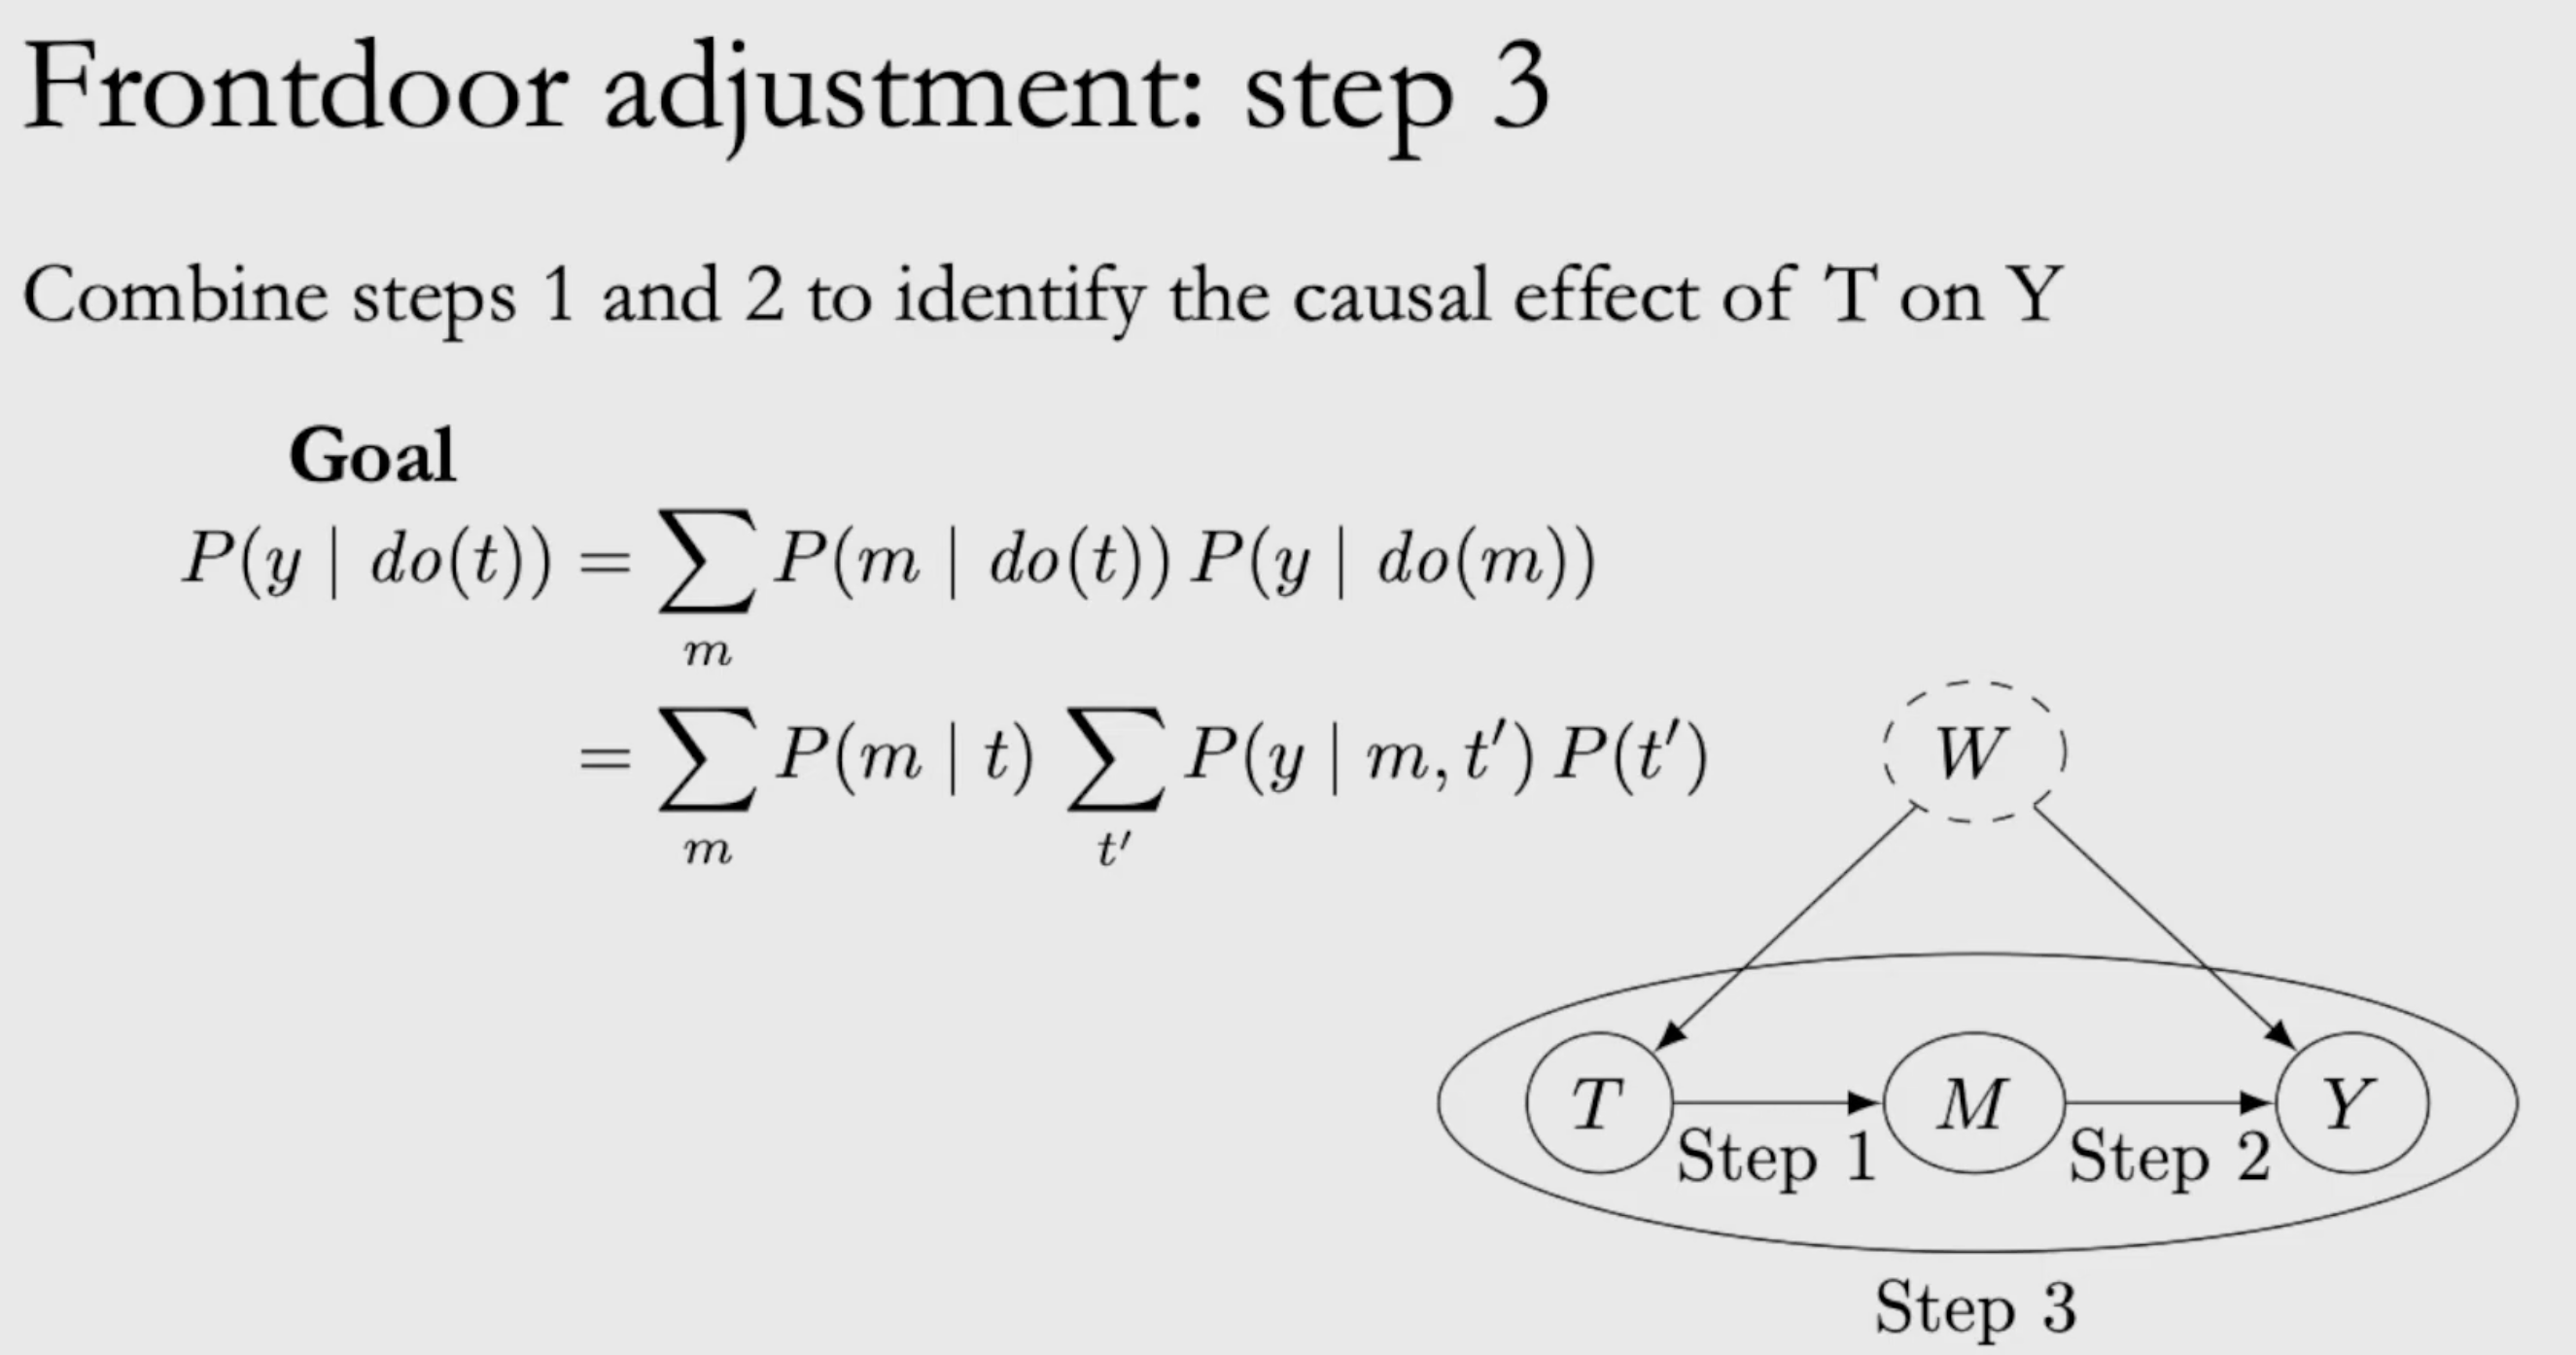
\includegraphics[width=250px]{draft-photos/frontdoor_adjustment_explanation3.png}
  \caption{Frontdoor Adjustment}
  \label{fig:frontdoor_adjustment_explanation3}
\end{figure}

\begin{figure}[H]
  \centering
  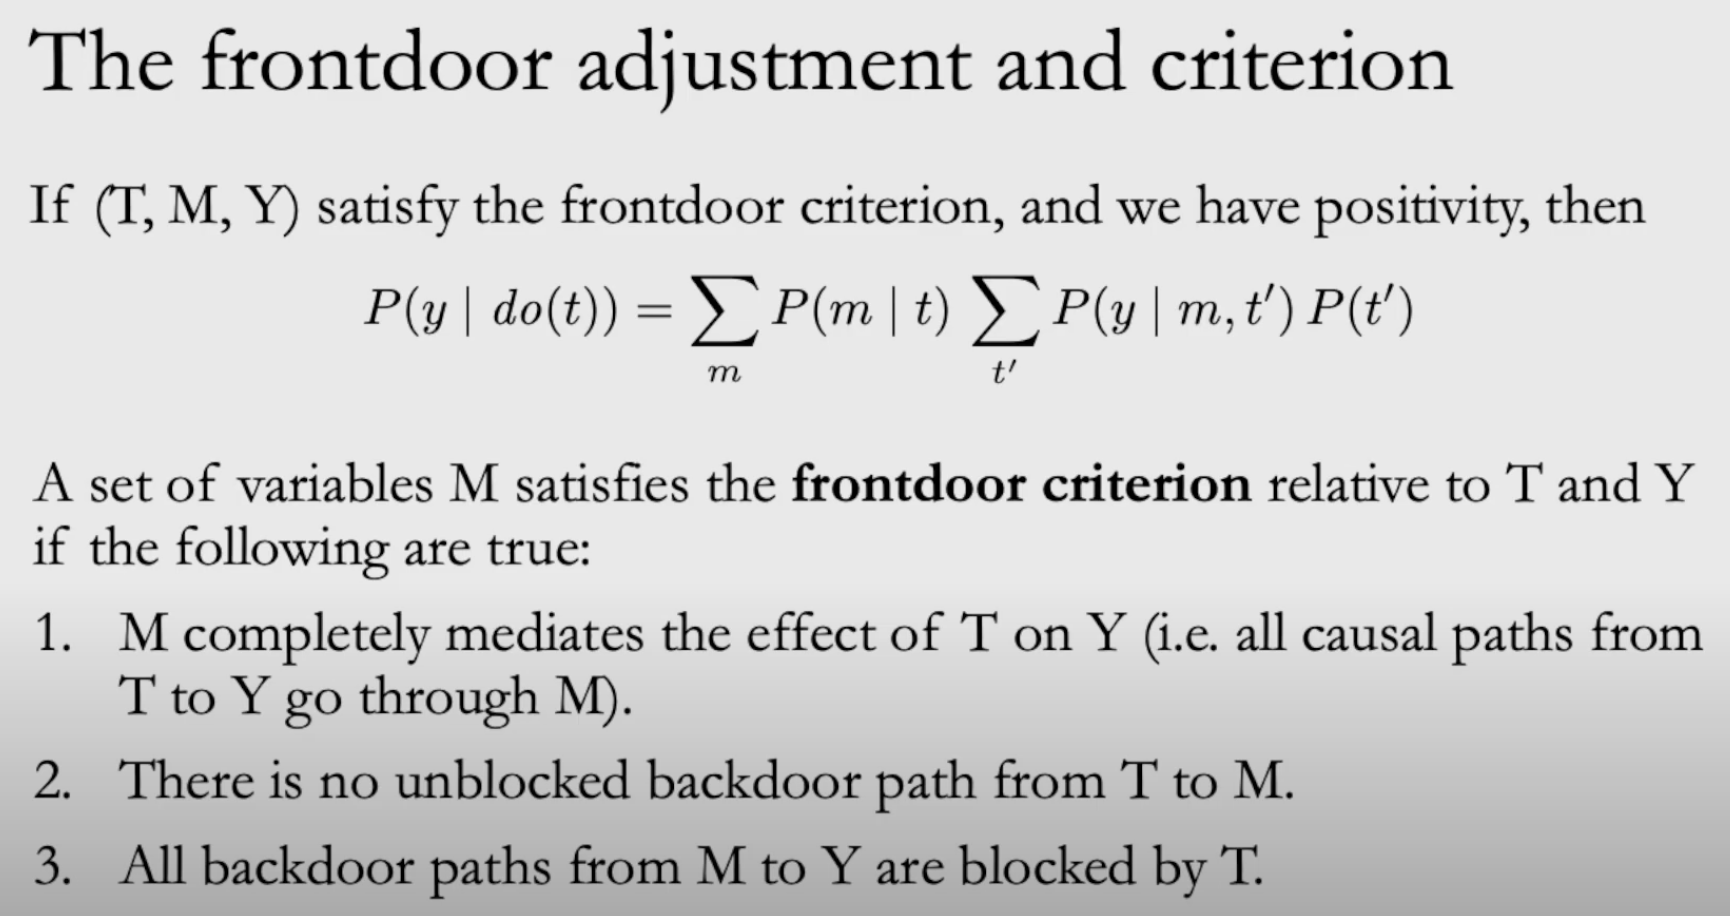
\includegraphics[width=250px]{draft-photos/frontdoor_adjustment_explanation4.png}
  \caption{Frontdoor Adjustment}
  \label{fig:frontdoor_adjustment_explanation4}
\end{figure}


\end{document}
